\chapter{Inputs to DAKOTA}\label{input}

\section{Overview of Inputs}\label{input:overview}

The DAKOTA executable supports a number of command line inputs, as
described in Section~\ref{tutorial:installation:running}.  Among
these are specifications for the DAKOTA input file and, optionally, a
restart file.  The syntax of the DAKOTA input file is described in detail 
in the DAKOTA Reference Manual~\cite{RefMan}, and the restart file is
described in Chapter~\ref{restart}.

The DAKOTA input file may be prepared manually (e.g., using a text
editor such as \texttt{xemacs} or \texttt{vi}), or it may be defined
graphically using the JAGUAR graphical user interface, as described in
Section~\ref{input:gui}.  Once prepared, the DAKOTA input file and/or
command line may identify additional files for data import as
described in Section~\ref{input:import}.

\section{JAGUAR 2.1}\label{input:gui}

JAGUAR (JAva GUi for Applied Research) is a Java software tool for
automatically rendering a graphical user interface (GUI) from a
structured input specification.  The dynamically-generated interface
enables users to create, edit, and externally execute analysis
application input files and then view the results.  JAGUAR is built on
top of the Eclipse Framework \cite{Eclipse} as an Eclipse Rich
Client Product, providing it the look, feel, and features of Eclipse
Applications.

JAGUAR serves as a GUI for DAKOTA.  It parses a DAKOTA NIDR input
specification and presents the user with linked graphical and plain
text representations of problem set-up and option specification for
DAKOTA studies. After the data have been input by the user, JAGUAR
generates one or more input files for DAKOTA; it can also execute
DAKOTA, capturing and (eventually) interpret the results.

JAGUAR 2.1 is available for Windows 32- and 64-bit platforms, 
Mac (Intel processors), and Linux 32- and 64-bit platforms. 
While JAGUAR's core source is BSD licensed,
binary distributions of JAGUAR include Eclipse Workbench components
and are therefore subject to the terms of the Eclipse Public License.
A short description of the steps for downloading, installing, and
executing JAGUAR is provided below.

\subsection{Downloading and Installing JAGUAR}

A short description of the steps for downloading and installing JAGUAR
is provided here.

\begin{itemize}
\item \textbf{Install supporting JAVA software} (if needed).  JAGUAR
  requires a Java Runtime Environment (JRE) version 5.0 or above. (Sun
  has revised its 1.X.X versioning system, and version 5.0 is the same
  as 1.5.0 in the old numbering scheme.)  If a Java Runtime
  Environment is not already installed on your machine, you will need
  to download and install a 5.0 JRE from:

\url{http://java.sun.com/j2se/1.5.0/download.jsp} 
{\small [click on ``Java Runtime Environment (JRE) 5.0 ...'']}

\item \textbf{Install JAGUAR}.  As per the DAKOTA download process
  described in Section~\ref{tutorial:installation:how1}, the JAGUAR
  distribution is accessed by clicking on the download link available
  from:~\url{http://dakota.sandia.gov/download.html} and
  filling out the short online registration form.  Download the JAGUAR
  install for your platform (Windows 32/64-bit, Mac, or Linux 32/64-bit).

The JAGUAR package is provided as a zipped archive file.  Windows and
Mac users should be able to double-click on the file's icon from a
file system browser to perform the extraction.  Linux users can use
the {\tt unzip} utility to unzip the archive from their command-line
console.  The JAGUAR installation package is self-contained, so JAGUAR
can be directly run immediately after extracting the archive. (See
Figure~\ref{fig:input:jag_package}.)  Take note of where you installed
as you may want to create a shortcut or link to the installed JAGUAR 
executable.
\begin{figure}
  \centering
  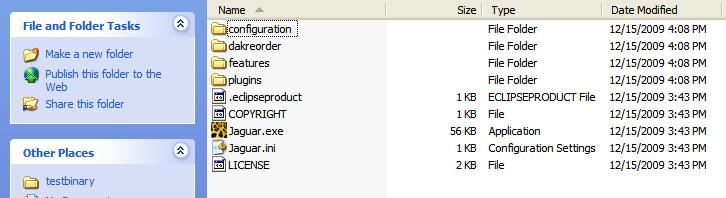
\includegraphics[scale=0.6]{images/jag_package}
  \caption{The JAGUAR installation package.}
  \label{fig:input:jag_package}
\end{figure}

\end{itemize}


\subsection{Running JAGUAR for the First Time}

When starting JAGUAR for the first time, you should see a ``Welcome''
screen.  As can be seen in Figure~\ref{fig:input:jag_welcome}, the
Welcome screen provides quick navigation to many JAGUAR features.
This screen can be closed at anytime by clicking on the ``X'' located
on the Welcome tab and returned to at anytime via the JAGUAR help menu
({\bf Help $\rightarrow$ Welcome}).
\begin{figure}
  \centering
  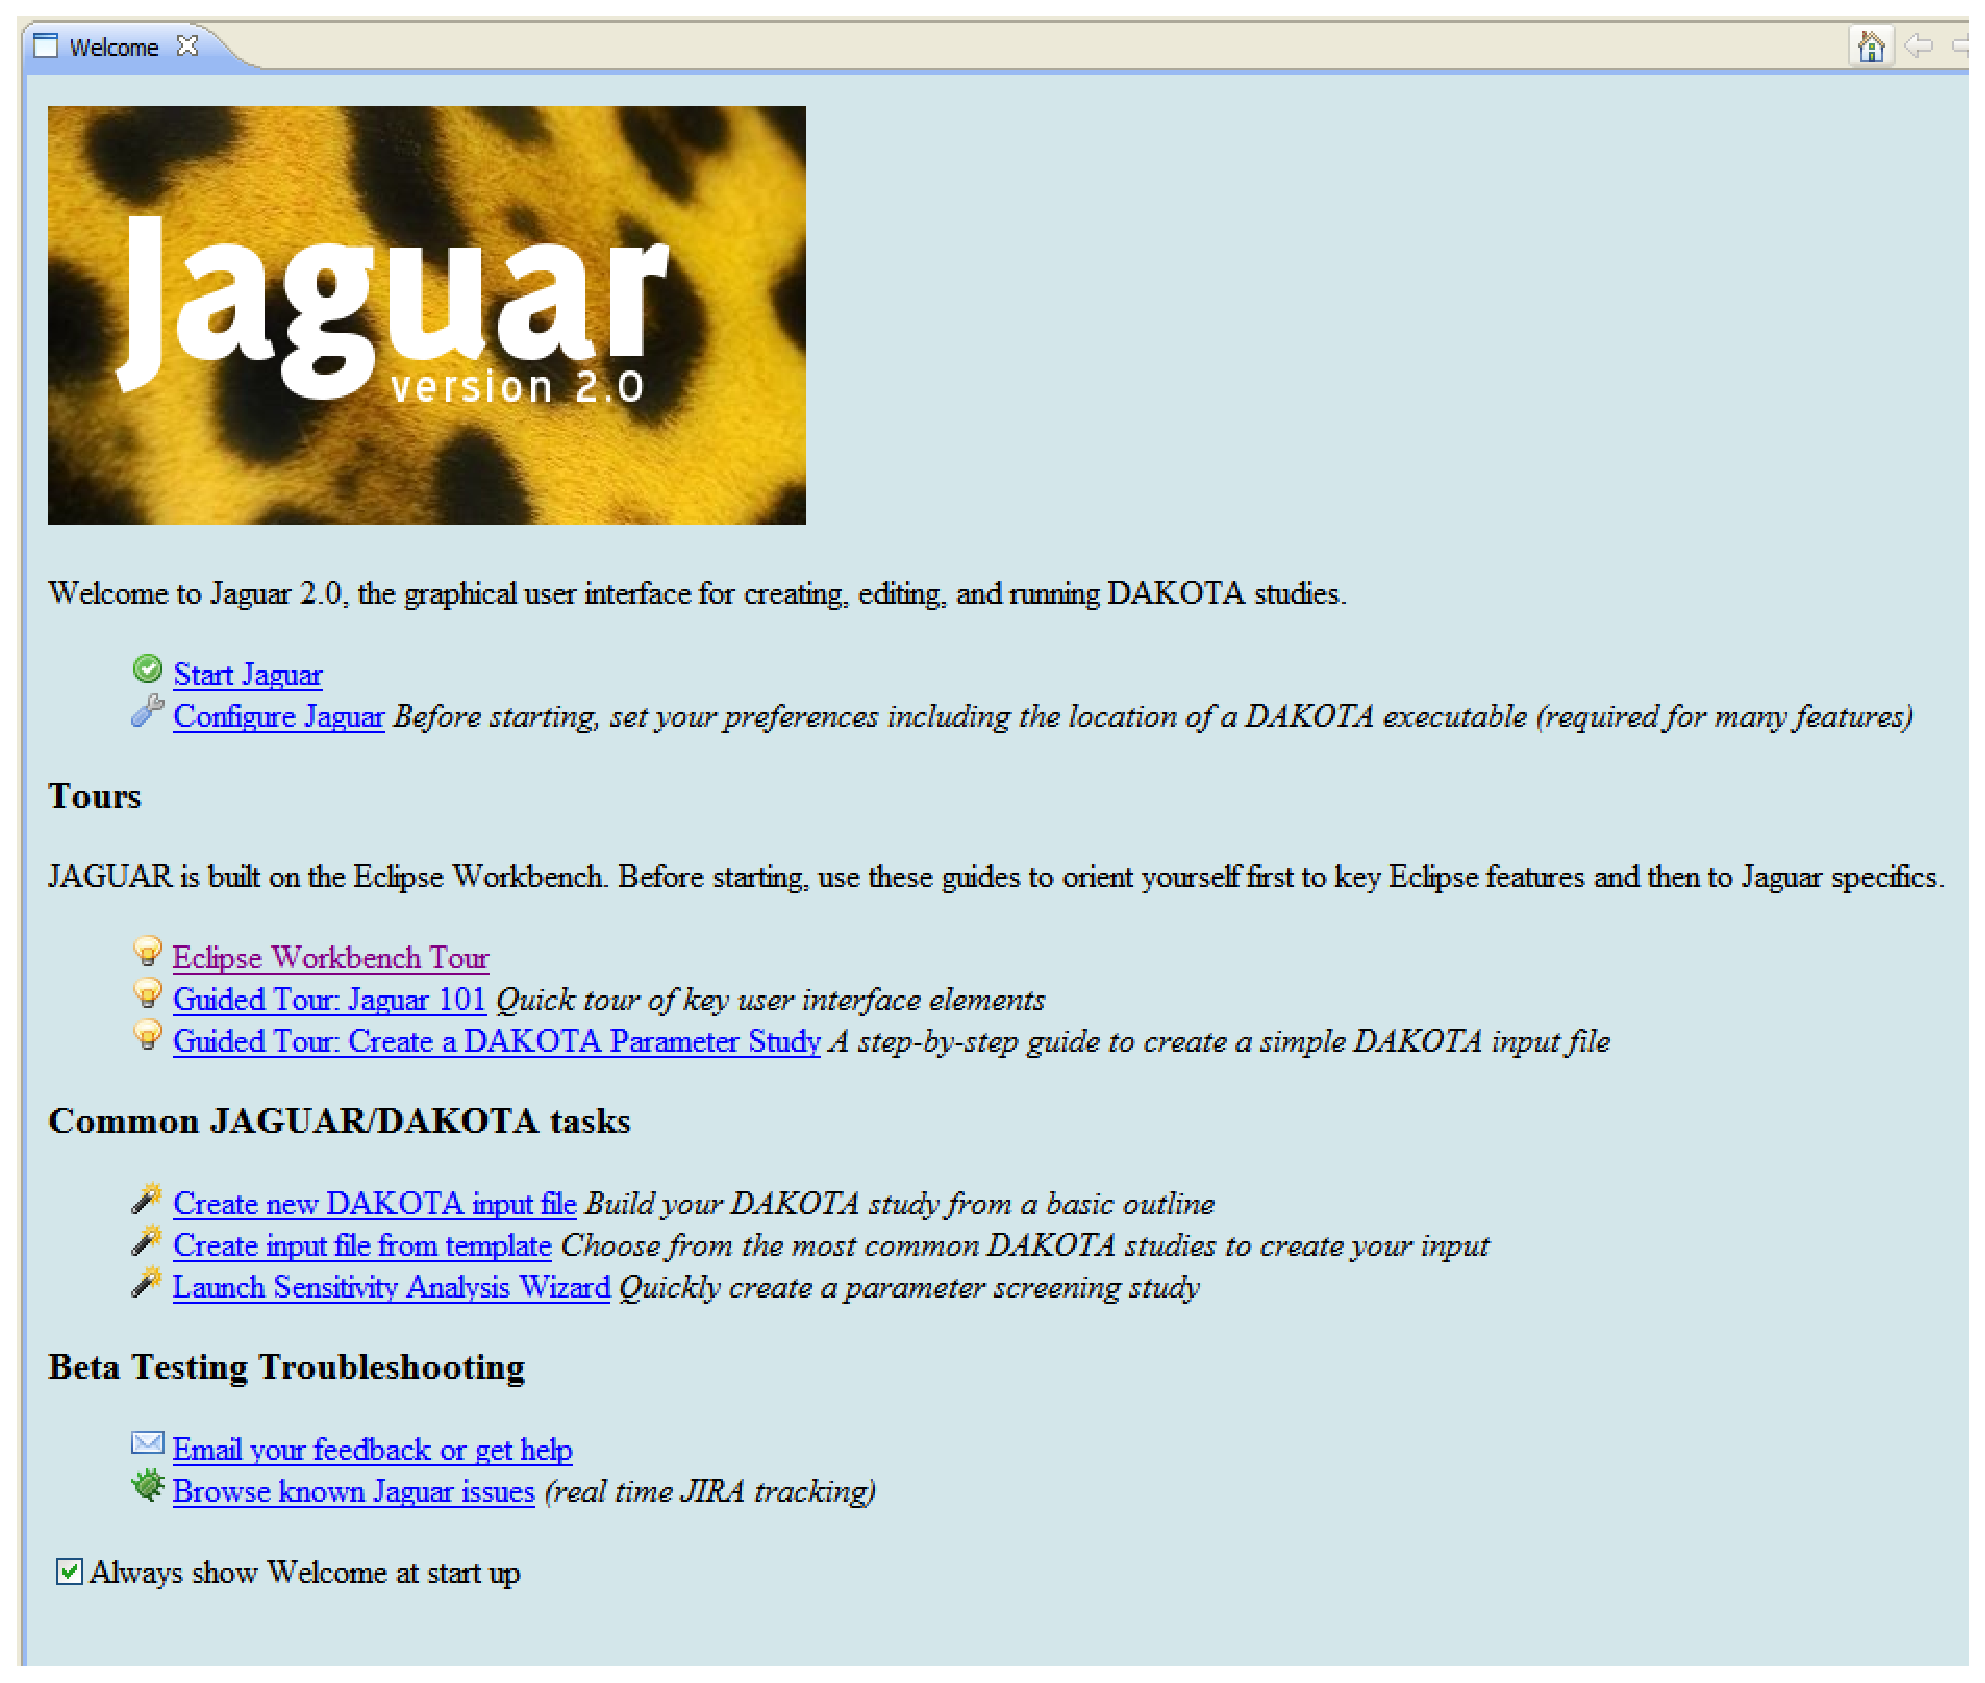
\includegraphics[scale=0.4]{images/jag_welcome}
  \caption{The JAGUAR ``Welcome'' screen.}
  \label{fig:input:jag_welcome}
\end{figure}

\begin{itemize}
\item {\bf Start Jaguar.}  The ``Start Jaguar'' link allows users to
  directly proceed to an empty JAGUAR interface.  

\item {\bf Tours.} The Tours section offers guides for beginning
users.  As JAGUAR is built on the Eclipse Workbench, new users will
benefit from the Eclipse Workbench Tour, a quick online reference for
Eclipse framework features like Views, Perspectives, etc.  The next
two links provides access to guided tours via JAGUAR Cheat Sheets
which are shown in Figure~\ref{fig:input:jag_cheatsheets}.
\begin{figure}
  \centering
  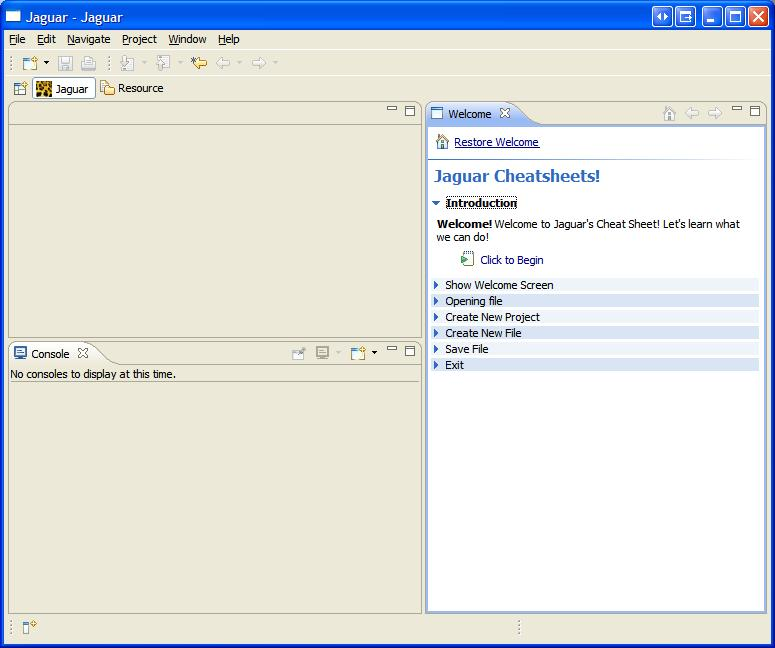
\includegraphics[scale=0.6]{images/jag_cheatsheets}
  \caption{A sample JAGUAR cheatsheet.}
  \label{fig:input:jag_cheatsheets}
\end{figure}
JAGUAR Cheat Sheets are a useful mechanism for quickly learning how to
perform important JAGUAR operations such as opening and saving files.
They utilize an interactive step-by-step approach to guide new users
through JAGUAR.  The Welcome screen is also accessible from Cheat
Sheets.  Cheat Sheets usually dock on the side of the application so
as to not obstruct user interactions, and can always be accessed from
the JAGUAR help menu ({\bf Help $\rightarrow$ Cheat Sheets}).

\item {\bf Create new input file.}  This link creates an empty DAKOTA
  input file.  New input files can also be accessed by selecting {\bf
    New $\rightarrow$ DAKOTA input file} from the File menu.  Users
  must enter a file name for newly-created input files when attempting
  to save them for the first time.

\item {\bf Create new input file from template.}  This links creates a
  new input file from existing DAKOTA templates.  Users must also
  enter a file name when saving these newly-created input files.  This
  action can also be accessed from the File menu by selecting {\bf New
  $\rightarrow$ DAKOTA input file from template}.

\end{itemize}

The remaining two links are used for sending an email to the JAGUAR
developers, and viewing existing JAGUAR bugs.


\subsection{Text Editors}

Figure \ref{fig:input:jag_texteditor} shows an example DAKOTA input
file in the JAGUAR text editor.  The text editor interface is the
first of two primary interfaces that JAGUAR contains for creating and
modifying DAKOTA input files.  For text-based editing, the ``Source''
tab toward the bottom of the JAGUAR window reveals the raw DAKOTA
input file text (likely only comfortable for experienced DAKOTA
users).
\begin{figure}
  \centering
  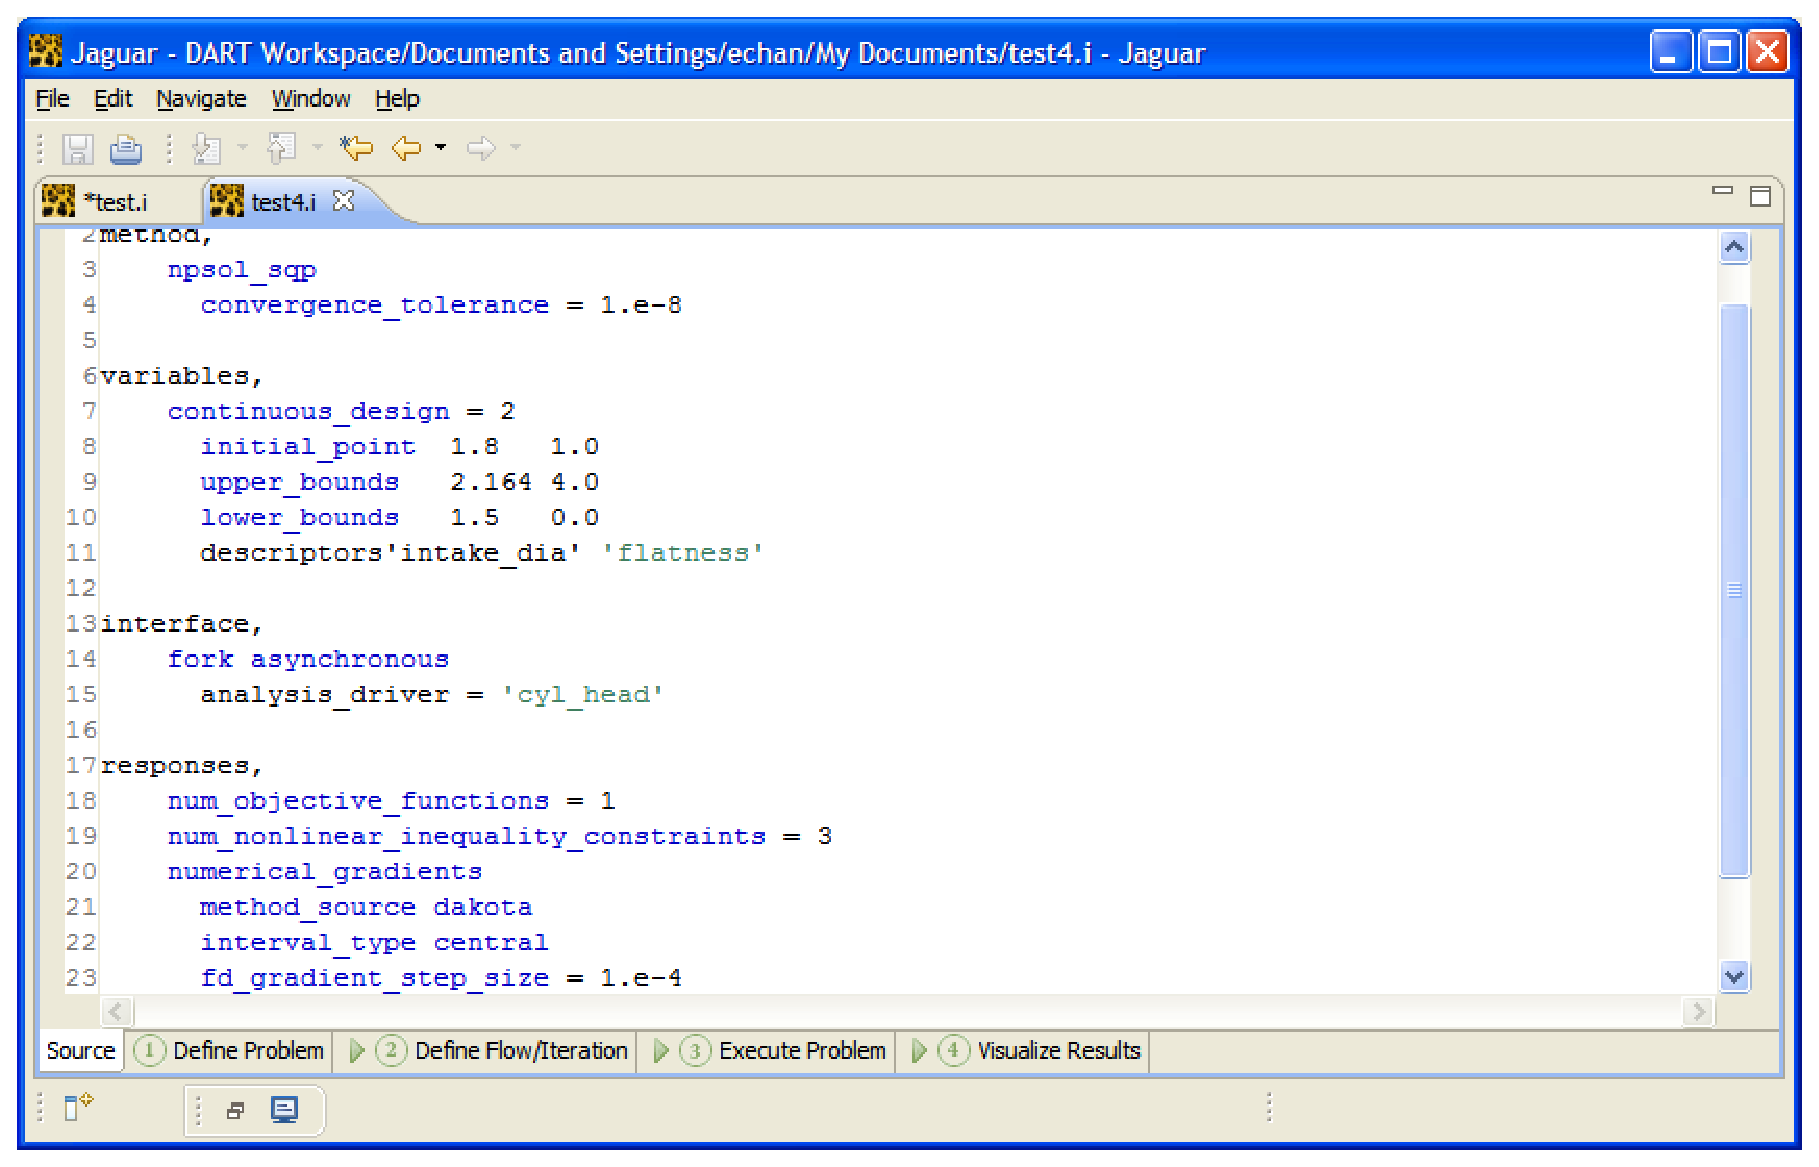
\includegraphics[scale=0.4]{images/jag_texteditor}
  \caption{The JAGUAR text editor.}
  \label{fig:input:jag_texteditor}
\end{figure}

This text editor supports simple syntax highlighting.  Additional text
editor features are syntax completion and context-sensitive, on-demand tooltip help.


\subsection{Graphical Editors}

JAGUAR's graphical editors are the second primary interface for
creating and modifying DAKOTA input files.  A unique feature of JAGUAR
is that the graphical user interface of these editors is {\em
dynamically} generated from the NIDR input specification for DAKOTA.
When your locally installed version of DAKOTA is updated, you can
point JAGUAR to the new version and it will re-render to match.

Graphical-based editing is conveniently separated into ``Define
Problem'' and ``Define Flow/Iteration'' sections; see the appropriate
tabs toward the bottom of the JAGUAR window in Figure
\ref{fig:input:jag_graphical1}.  ``Define Problem'' is where the
problem to iterate on is defined in terms of models, which map
variables through interfaces to responses.  ``Define Flow/Iteration''
is where a method or methods and possibly a strategy are specified.
\begin{figure}
  \centering
  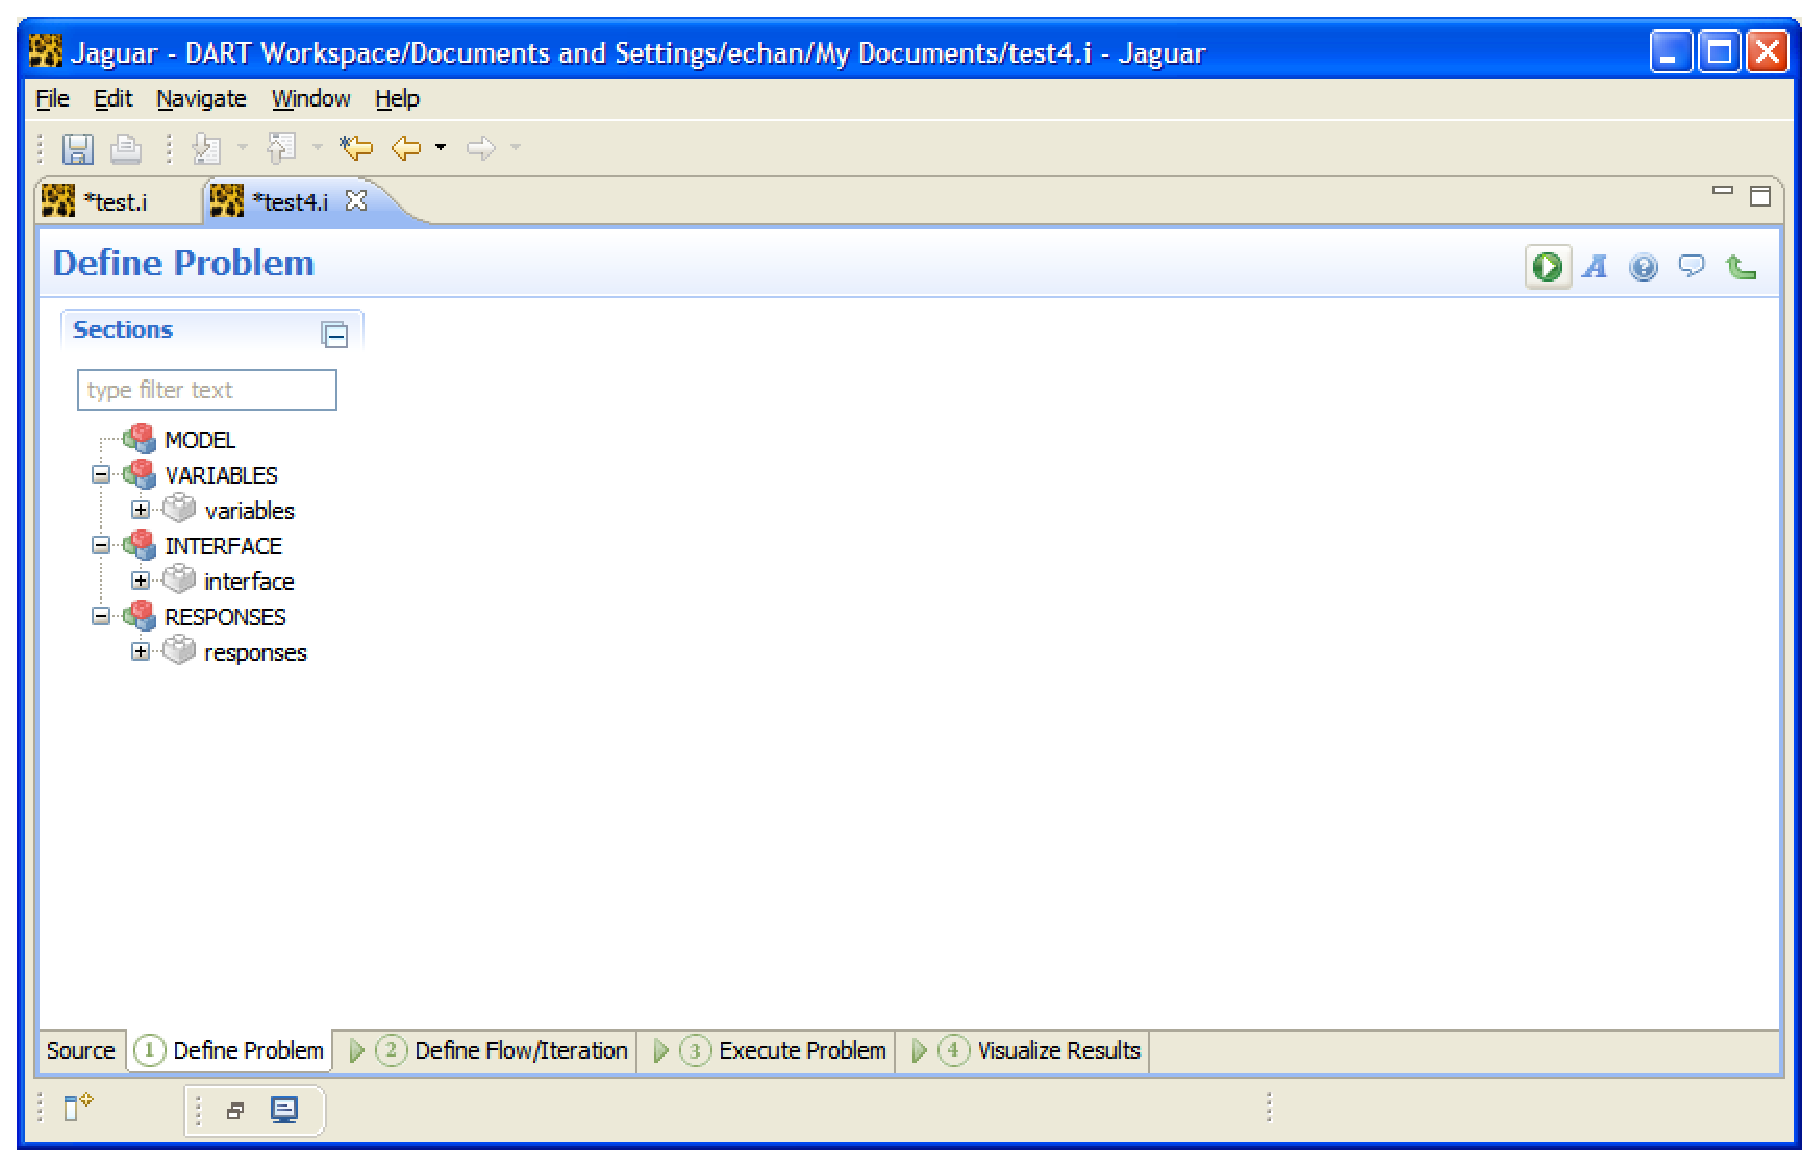
\includegraphics[scale=0.4]{images/jag_graphical1}
  \caption{The ``Define Problem'' portion of the JAGUAR graphical
    editor.}
  \label{fig:input:jag_graphical1}
\end{figure}

Each pane in the graphical view has two components.  On the left is
the tree hierarchy, which provides users with easy navigation across
the structured input file.  The right side of the view is where
content is displayed and selections may be made.  As an example, see
Figure \ref{fig:input:jag_graphical2}.
\begin{figure}
  \centering
  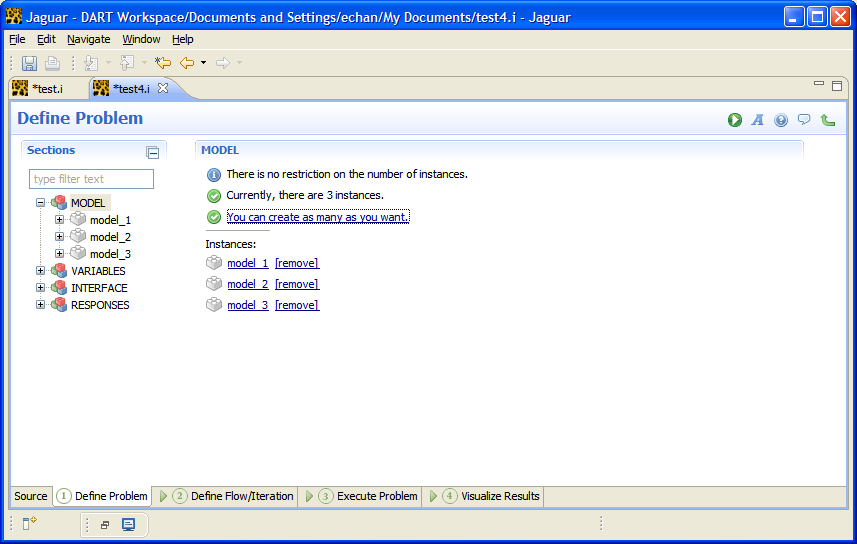
\includegraphics[scale=0.4]{images/jag_graphical2}
  \caption{Content selected from the left tree hierarchy is displayed
    on the right side of the view.}
  \label{fig:input:jag_graphical2}
\end{figure}

When a top-level element (i.e., Model, Variable Interface, Responses,
Strategy, or Method), represented by a multi-colored brick, is
selected by a user, the right pane will display a top-level overview
of the selection.  From this page, certain top-level elements will
show instance restrictions for a valid input file, allow the user to
create a new instance, and to go directly to or delete an existing
instance.

Within each top-level instance lie unique instances (represented by a
gray brick).  Each instance contains many possible configurable
settings, which are all organized according to their hierarchy as
shown in Figure \ref{fig:input:jag_graphical3}.  We call these
``elements.''
\begin{figure}
  \centering
  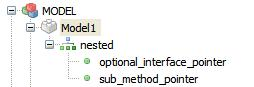
\includegraphics[scale=0.8]{images/jag_graphical3}
  \caption{An organized hierarchy of possible configurable settings.}
  \label{fig:input:jag_graphical3}
\end{figure}

When an instance is selected, its elements are displayed in the right
content pane. (See Figure \ref{fig:input:jag_graphical4}.)  Note that
certain elements have nested elements, which are not immediately
displayed in the content pane.  To view these child elements, select
the element in the left hierarchy tree.
\begin{figure}
  \centering
  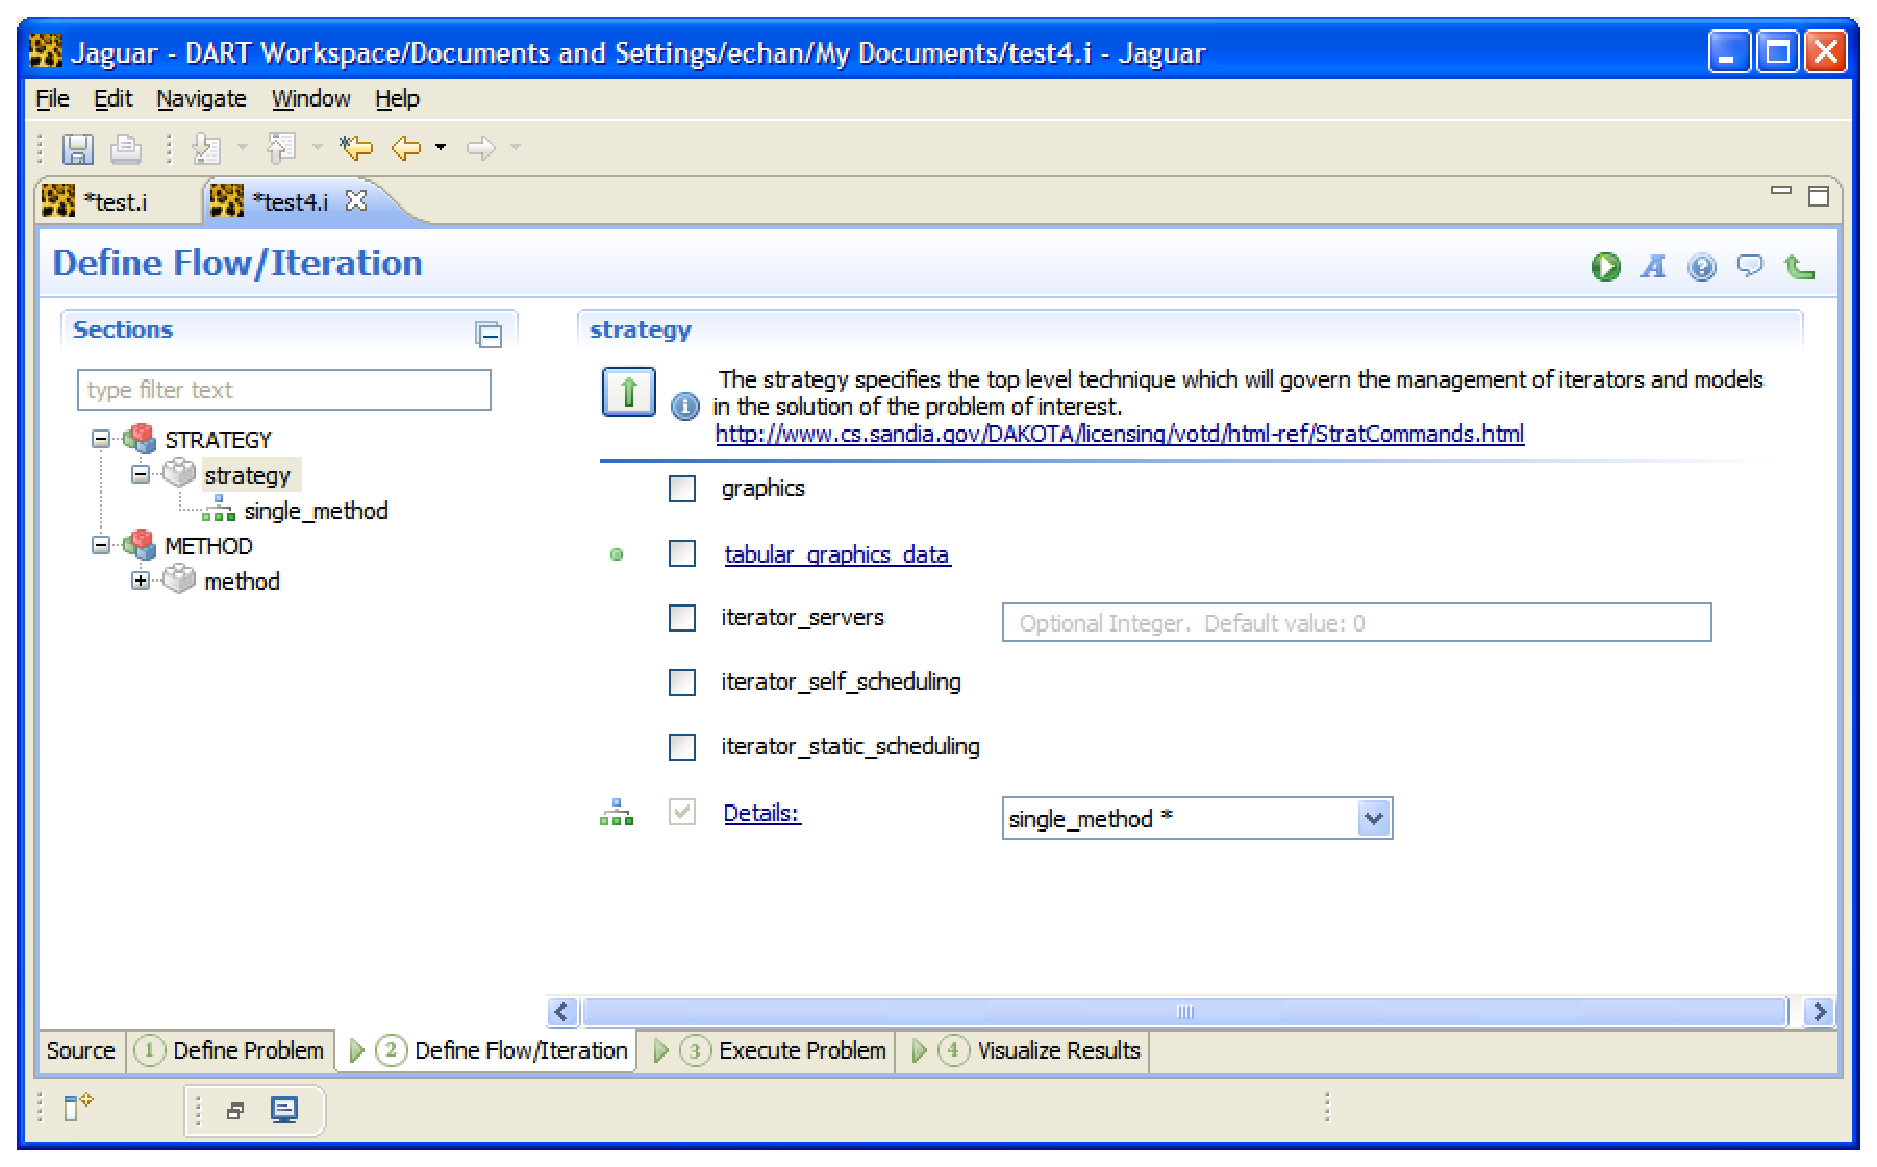
\includegraphics[scale=0.4]{images/jag_graphical4}
  \caption{Display of elements from a selected instance.}
  \label{fig:input:jag_graphical4}
\end{figure}

There are five basic types of elements in JAGUAR.
\begin{enumerate}
\item The first is an element without a value.  In Figure
  \ref{fig:input:jag_graphical5}, notice the checkbox to the left of
  the element; this allows the user to enable and disable the element.
  Only enabled elements are represented in the input file, which of
  course can be viewed in the ``Source'' representation (i.e., the
  JAGUAR text editors).  Note that some elements are required, and
  thus cannot be disabled.
\begin{figure}
  \centering
  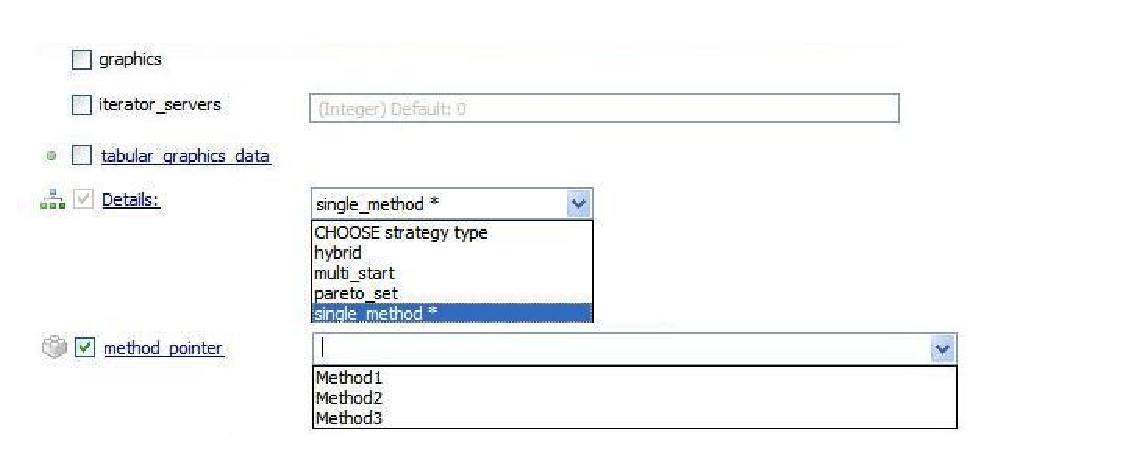
\includegraphics[scale=0.8]{images/jag_graphical5}
  \caption{Different element types in JAGUAR.}
  \label{fig:input:jag_graphical5}
\end{figure}

\item The second element type allows users to set values of type
  Integer, Real, String, or a space-delimited list.

\item Nested elements are supported in JAGUAR, and are indicated by a
  green bullet and the presence of a hyperlink.  Selecting a hyperlink
  is one way to view the nested element in the right-side content
  pane.  The up arrow allows quick return to a parent element in the
  problem specification.

\item Drop-down lists in JAGUAR are indicated by a choice icon.  When
  the list is selected, it behaves like one of the former three
  element types.  In terms of drop-down lists' contents, note that the
  first element functions as a header text whose purpose is to aid the
  user's selection of an appropriate element below.  Asterisks are
  also used to indicate the default element of the list.

\item The fifth and final element is a pointer element that allows the
  reference of other existing elements.  Hyperlinks allow users to
  quickly view that instance in the content pane.  In addition, when
  an unrecognized instance name is manually entered in a pointer
  element, JAGUAR automatically creates that new instance.

\end{enumerate}

Push-up elements allow sub-specifications to be displayed in the
current pane instead of requiring a dive in the tree to see them.
Figures~\ref{fig:input:jaguar_pushup_on}
and~\ref{fig:input:jaguar_pushup_off} show JAGUAR with push-up
elements on (default) and off, respectively.  Control behavior of
push-ups with the upward facing arrow on the top right of the editor
or in preferences.

\begin{figure}
  \centering
  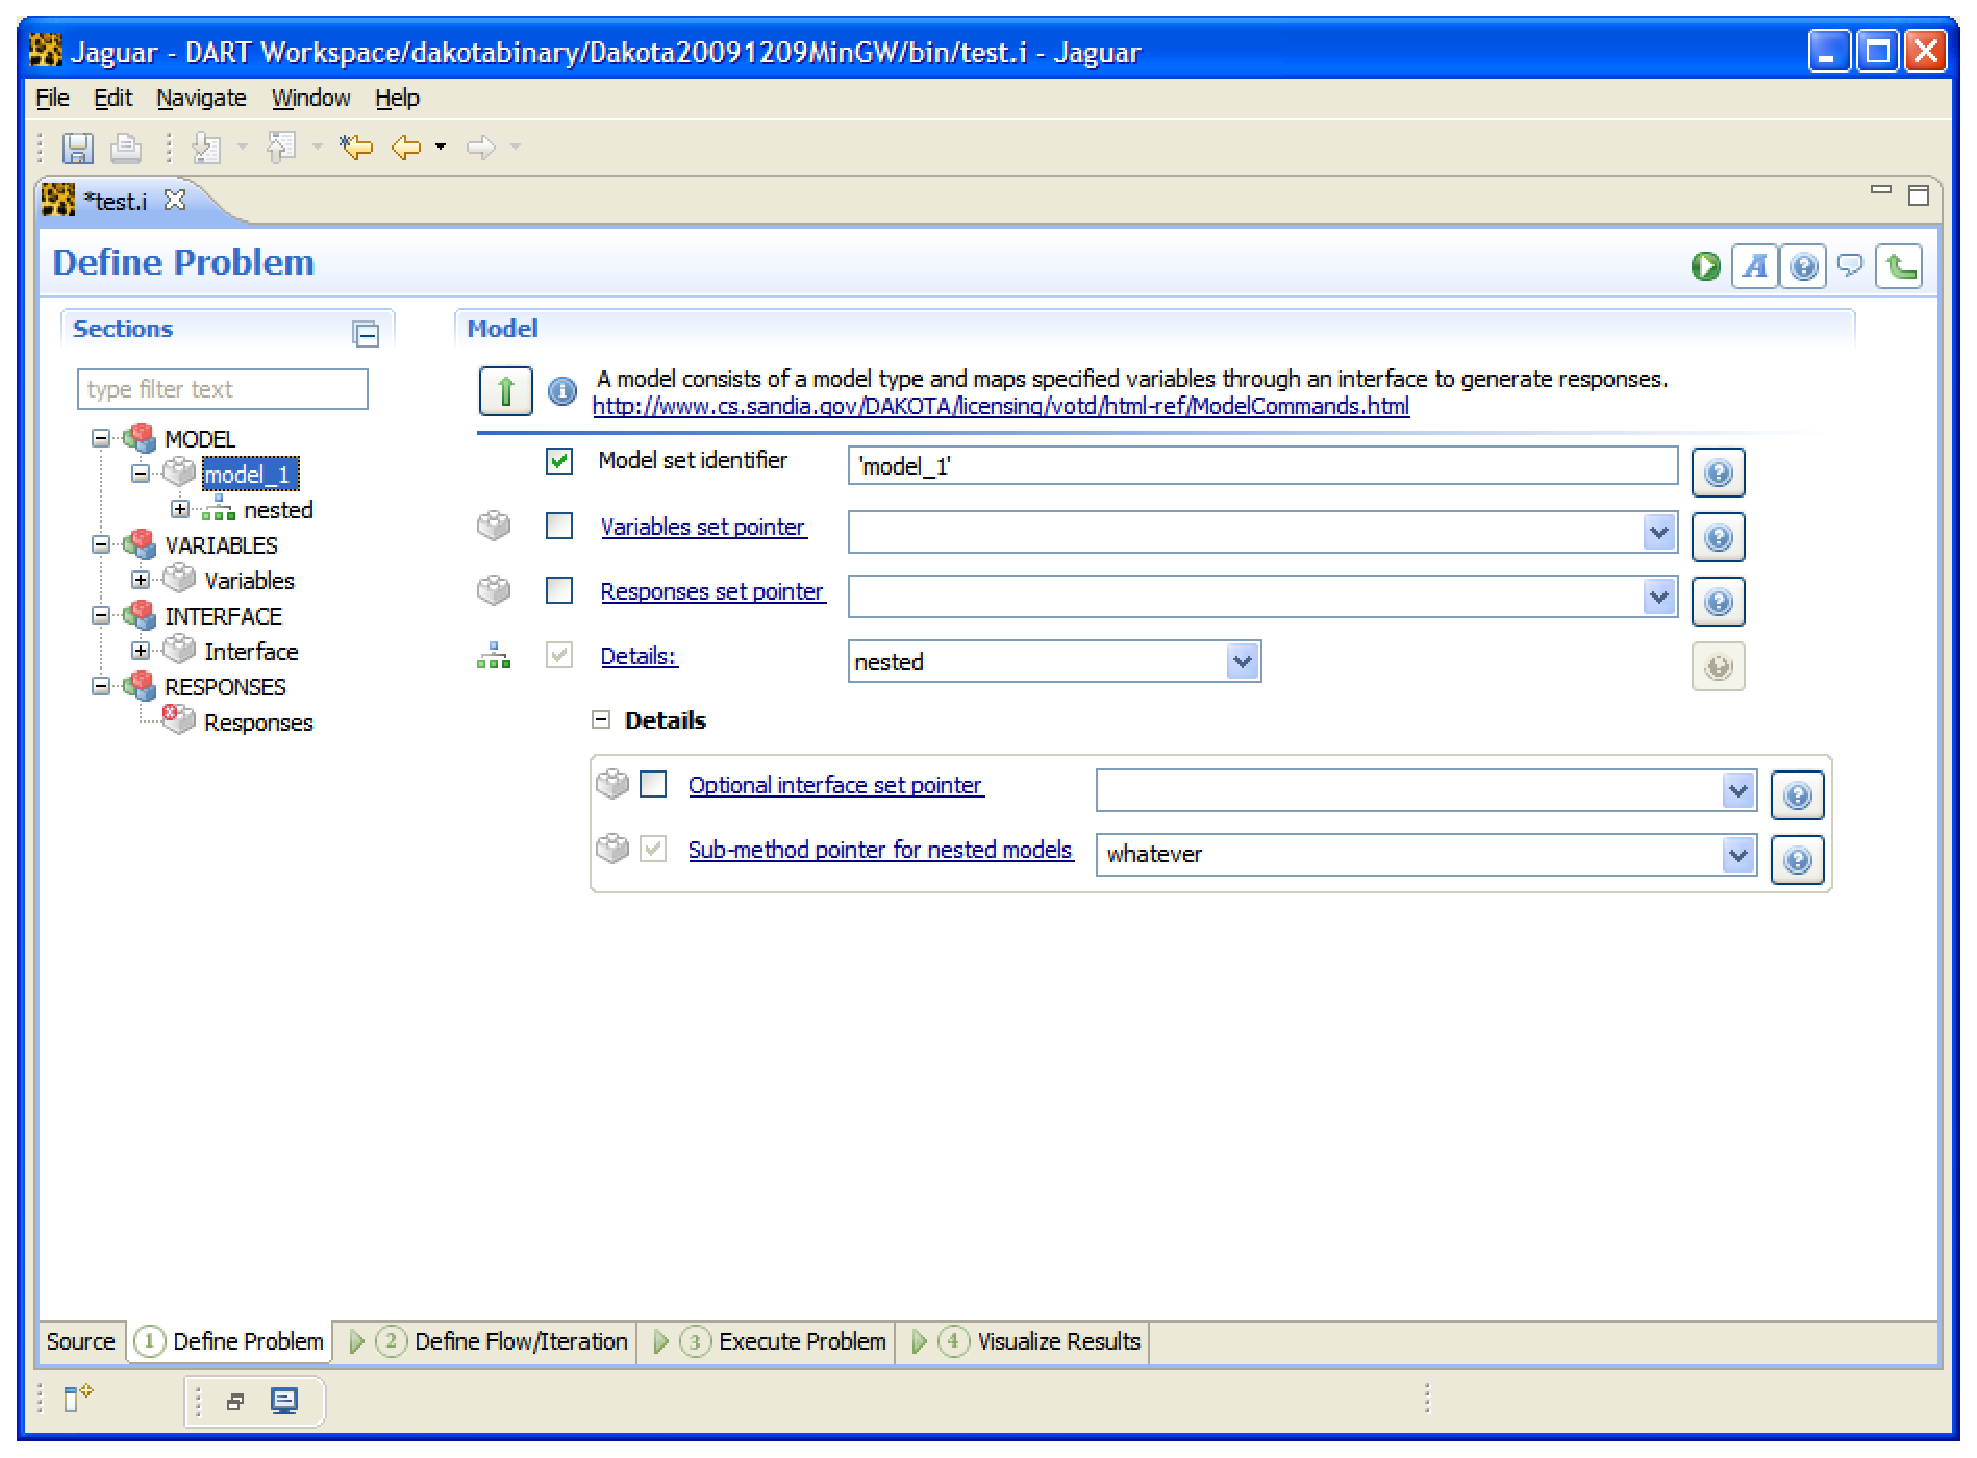
\includegraphics[scale=0.4]{images/jaguar_pushup_on}
  \caption{JAGUAR with push-up elements enabled (default).}
  \label{fig:input:jaguar_pushup_on}
\end{figure}

\begin{figure}
  \centering
  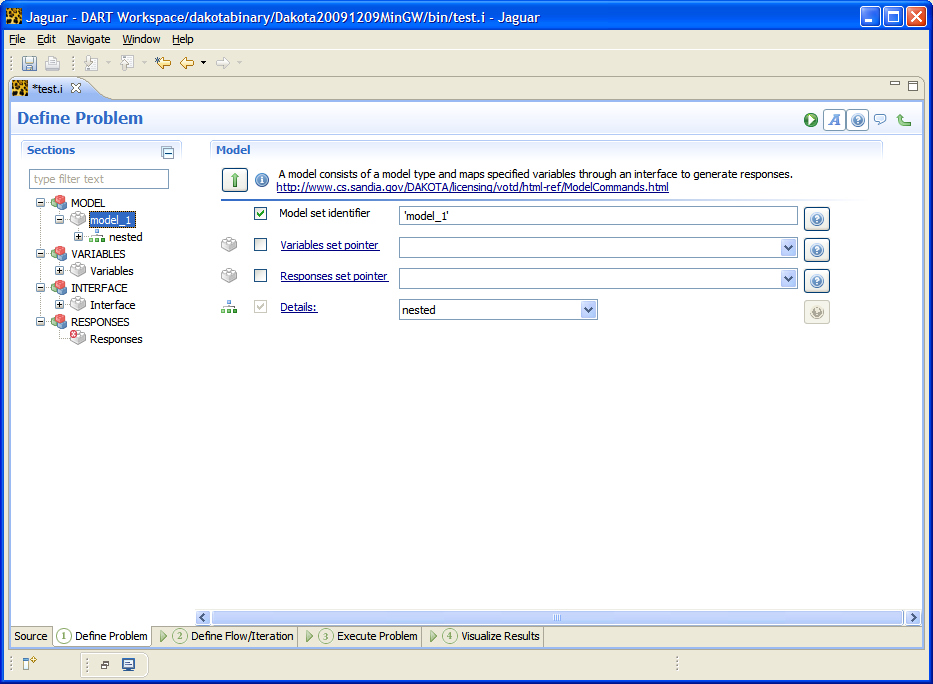
\includegraphics[scale=0.4]{images/jaguar_pushup_off}
  \caption{JAGUAR with push-up elements disabled.}
  \label{fig:input:jaguar_pushup_off}
\end{figure}

The JAGUAR toolbar, shown in Figure~\ref{fig:input:jaguar_toolbar}
offers (from left to right) quick access for running DAKOTA input
files, displaying pretty names instead of keywords, toggling help
text, displaying comments, and toggling push-up elements.

\begin{figure}
  \centering
  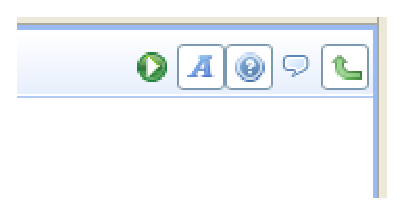
\includegraphics[scale=0.4]{images/jaguar_toolbar}
  \caption{JAGUAR toolbar for running DAKOTA or toggling many
  options.}
  \label{fig:input:jaguar_toolbar}
\end{figure}


\subsection{DAKOTA Execution}

The ``Execute Problem'' tab contains several options for executing
DAKOTA on the active input file, as shown in
Figure~\ref{fig:input:jag_execute}.
\begin{figure}[htbp]
  \centering
  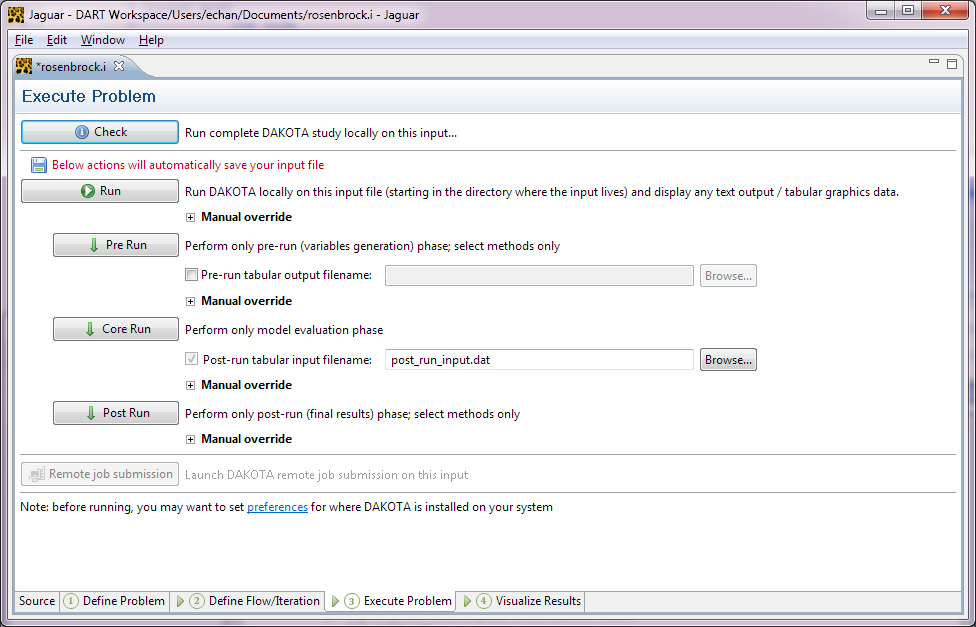
\includegraphics[scale=0.6]{images/4ExecuteProblem}
  \caption{The JAGUAR ``Execute Problem'' tab.}
  \label{fig:input:jag_execute}
\end{figure}
The execute options all rely on a locally installed copy of DAKOTA,
the path to which can be set via {\bf Window $\rightarrow$ Preferences $\rightarrow$ Jaguar}.

Currently five modes of DAKOTA execution are supported:
\begin{itemize}

\item {\bf Check:} While JAGUAR includes considerable input
validation, additional validation is managed solely by DAKOTA's input
parser.  To use DAKOTA to validate the active input file (via {\tt
dakota -check}), click the Check button and view the console output on
the Visualize tab.  You should see a message indicating that the check
completed and should see no errors
\begin{small}
\begin{verbatim}
Input check completed: problem specification parsed and objects instantiated.
\end{verbatim}
\end{small}

\item {\bf Run:} The run feature supports running DAKOTA on the local
machine using the active input file.  Clicking Run will start DAKOTA
in the same directory as the input file, so any necessary driver
scripts or data files must be present.  View the output from DAKOTA in
the console window:

\begin{verbatim}
<<<<< Iterator multidim_parameter_study completed.
<<<<< Function evaluation summary: 25 total (25 new, 0 duplicate)
<<<<< Best data metrics not defined for generic response functions
<<<<< Single Method Strategy completed.
\end{verbatim}

\item {\bf Pre Run:} Pre-run is a component of the normal DAKOTA run
process.  For select analyzer methods only, e.g., parameter studies
and sampling methods, DAKOTA supports a pre-run mode ({\tt dakota
-pre\_run}), which will generate the set of points at which DAKOTA
will evaluate the model and optionally write them to a tabular file.
The optional checkbox permits saving this generated file.  A
successful pre-run will terminate with a message:

\begin{small}
\begin{verbatim}
Pre-run phase complete: variables written to tabular file my_vars.dat
\end{verbatim}
\end{small}

\item {\bf Post Run:} Post-process user-supplied variables and
function evaluation data, for example, to compute final statistics in
a screening study (the analysis counterpart complementing Pre Run).
Pre-run and post-run are central to the sensitivity analysis wizard.

\item {\bf Core Run:} Perform only the model evaluation (invoke {\tt
analysis\_drivers}) to map variables to responses.  ({\tt dakota
-run})

\end{itemize}

Results from any execute option are displayed on the ``Visualize
Results'' tab as shown in Figure~\ref{fig:input:jaguar_visualize}.

\begin{figure}[htbp]
  \centering
  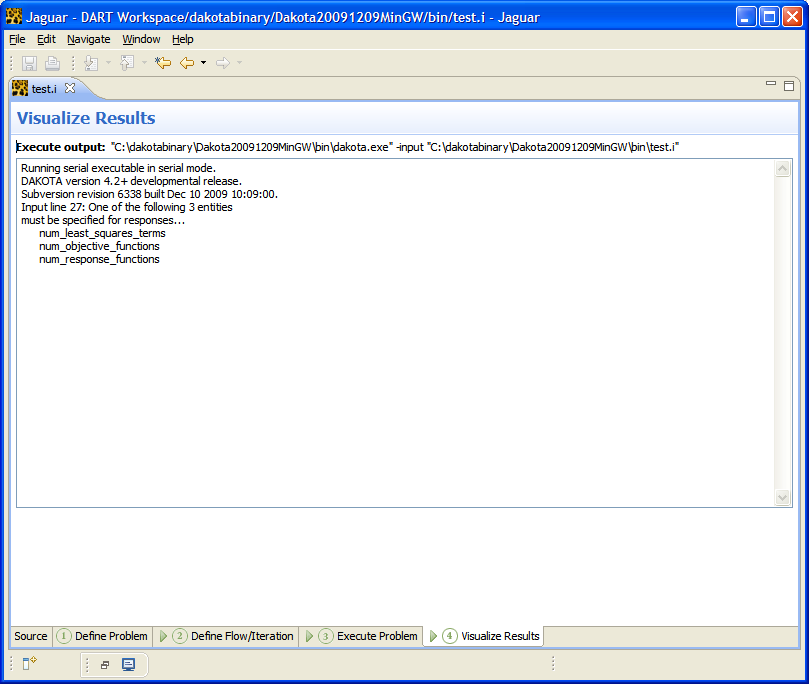
\includegraphics[scale=0.4]{images/jaguar_visualize}
  \caption{JAGUAR Visualize Results tab.}
  \label{fig:input:jaguar_visualize}
\end{figure}


For all problem execition supported modes under {\bf Run} the additional feature of 
{\bf Manual override} has been added to allow DAKOTA users to modify the problem execution 
commands on the fly, without having to open new files in JAGUAR and start from scratch. 


In future JAGUAR releases we plan to add another execute mode, the {\bf Remote job submission} for the users to be able to submit a DAKOTA job on a remote
compute cluster and monitor the job status.


\subsection{Sensitivity Analysis Wizard}

JAGUAR will ultimately provide wizards for creating customized DAKOTA
input files for a variety of common tasks such as optimization,
parameter estimation, and uncertainty quantification.  Presently, one
such wizard exists for creating a Latin hypercube sampling sensitivity
analysis (screening) study, and is accessible from the Welcome screen
and the main File menu ({\bf New $\rightarrow$ Sensitivity Analysis
Wizard}).

Upon launching, select either the variables definition (pre-run) phase
or analysis (post-run) phase (Figure~\ref{fig:input:jaguar_sa_wizard})
\begin{figure}
  \centering
  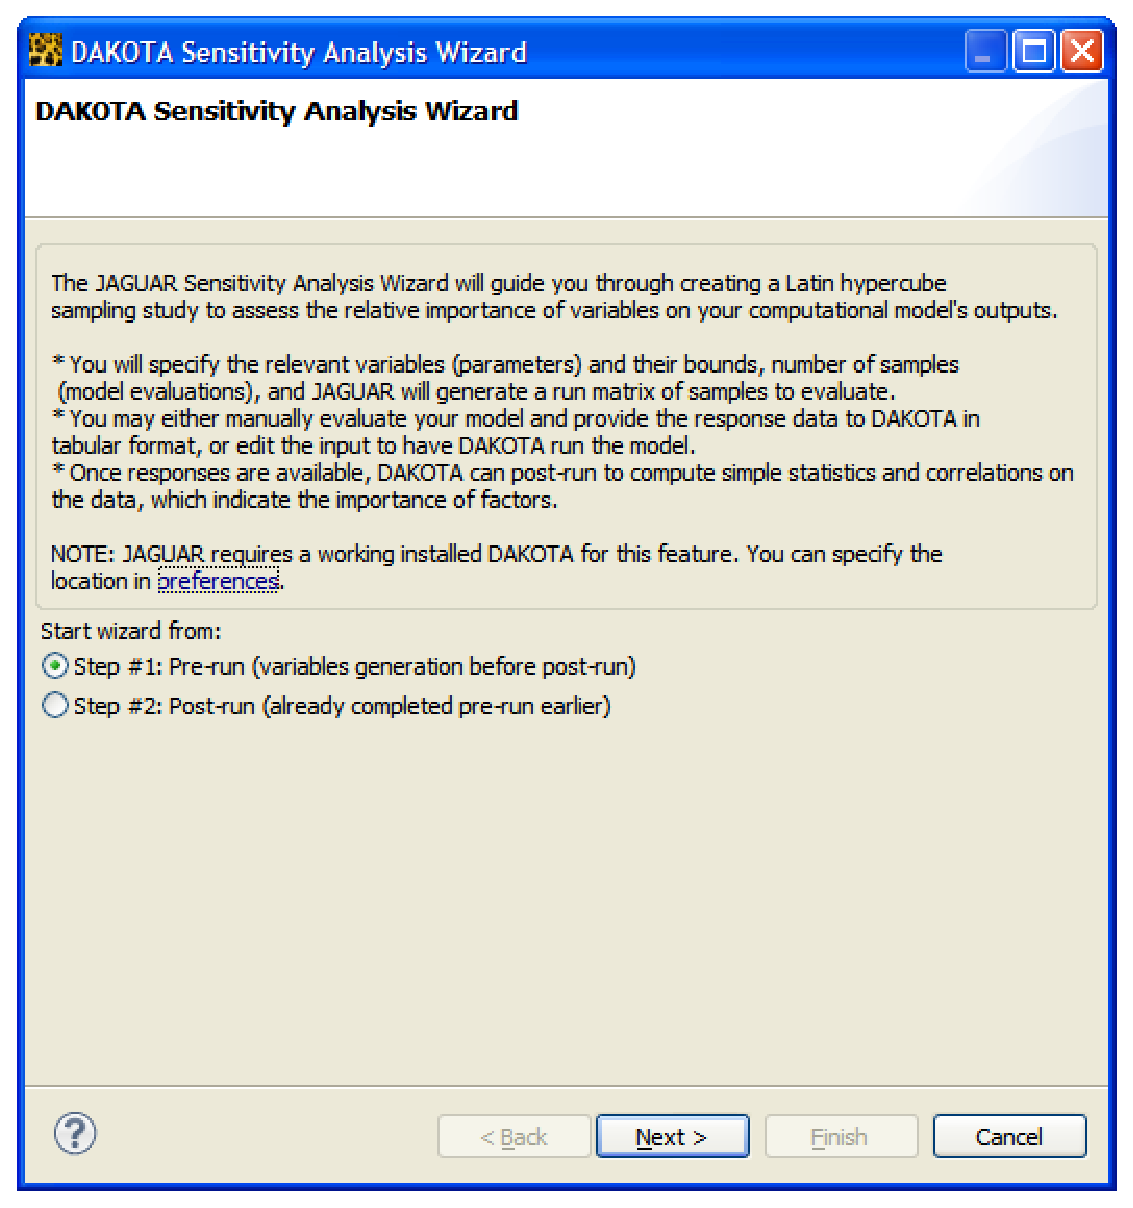
\includegraphics[scale=0.5]{images/jaguar_sa_wizard}
  \caption{The splash page for the JAGUAR Sensitivity Analysis
  Wizard.}
  \label{fig:input:jaguar_sa_wizard}
\end{figure}

Figure~\ref{fig:input:jag_wizard3} shows the second page of the
sensitivity analysis wizard.  The number of samples, uncertain
(uniformly-distributed) variables, and responses must be specified.
For each specified variable, lower and upper bounds are required;
there are also optional fields for specifying descriptors for each
variable.  After these fields have been complete, the user can
generate the LHS samples in the form of a run matrix using the
``Generate samples'' option, and/or save the input file for the LHS
study using the ``Save input file'' option and specifying a location
for the input file. (Selecting ``Save input file'' will end the
wizard.)
\begin{figure}
  \centering
  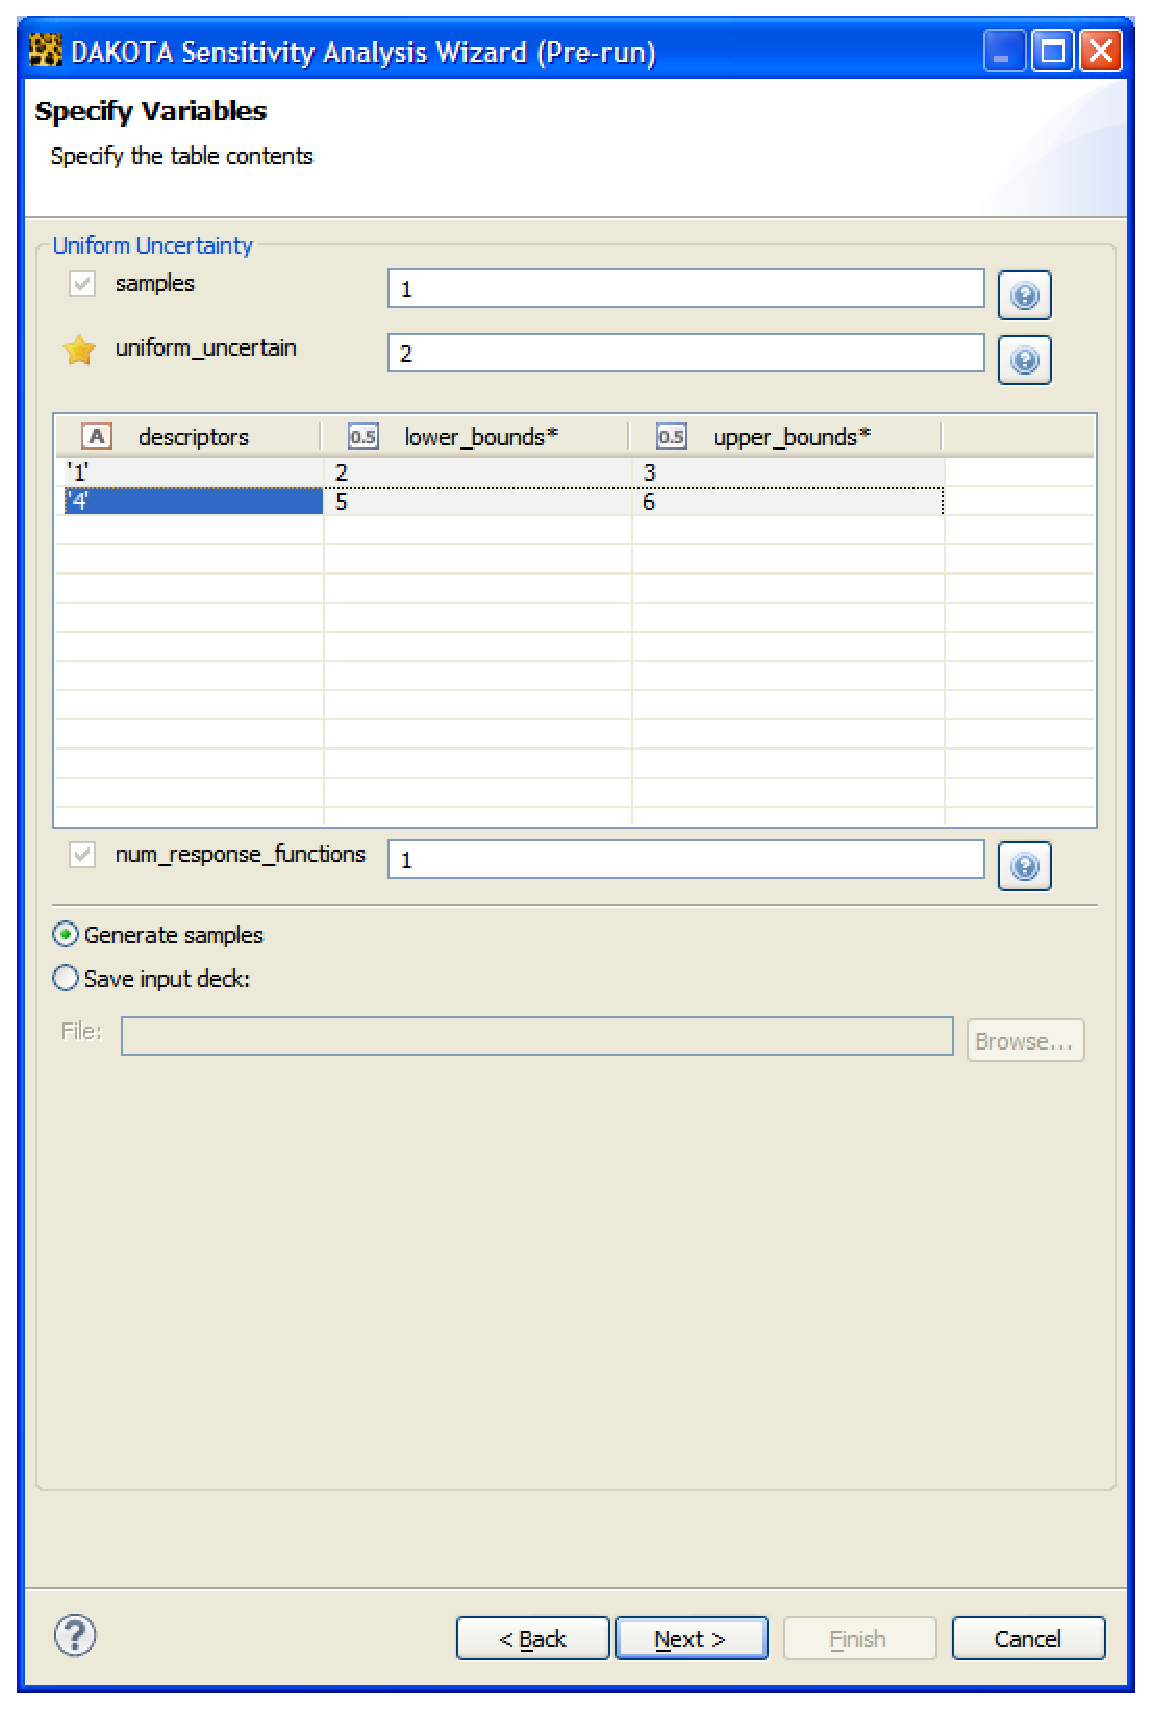
\includegraphics[scale=0.5]{images/jag_wizard3}
  \caption{The second page of the JAGUAR Sensitivity Analysis Wizard,
  pre-run phase.}
  \label{fig:input:jag_wizard3}
\end{figure}

Figure~\ref{fig:input:jag_wizard4} shows an example of the final page
of the wizard containing the generated run matrix if the ``Generate
samples'' option is selected.  Note that this option actually executes
the locally-installed version of DAKOTA (in ``pre-run'' mode) to
generate the run matrix.  The page also provides options for saving
both the input file and the generated run matrix.
\begin{figure}
  \centering
  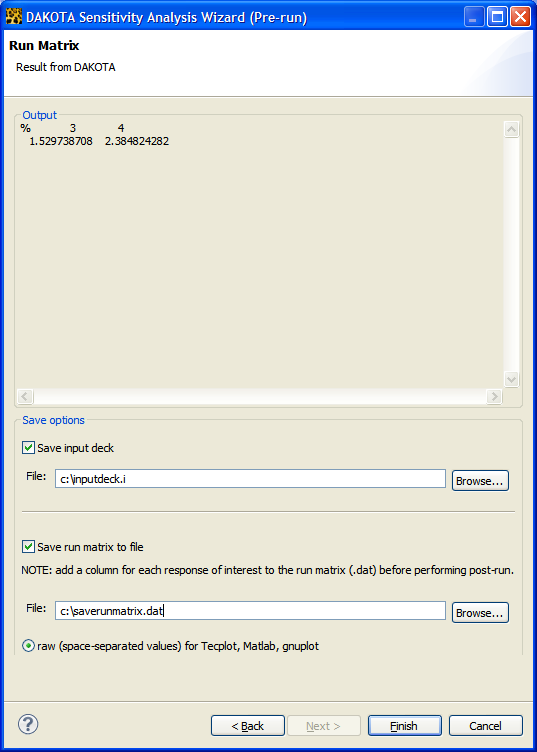
\includegraphics[scale=0.5]{images/jag_wizard4}
  \caption{The final page of the Sensitivity Analysis Wizard, pre-run
  phase.}
  \label{fig:input:jag_wizard4}
\end{figure}

After creating a samples file (run matrix), a use may either add
columns for response data to the file, or run DAKOTA to perform
variable to response mappings, then return to the wizard's post-run
mode.  Figure~\ref{fig:input:jaguar_sa_post_run} shows specification
of the saved input deck from pre-run and the location of the data file
containing the variables and response data to analyze.
\begin{figure}
  \centering
  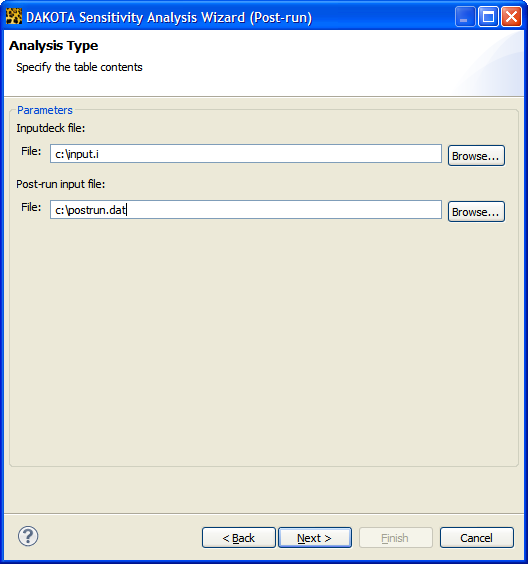
\includegraphics[scale=0.5]{images/jaguar_sa_post_run}
  \caption{The second page of the JAGUAR Sensitivity Analysis Wizard,
  post-run phase.}
  \label{fig:input:jaguar_sa_post_run}
\end{figure}

\subsection{Generating Input Files from Templates}

There exist many example input files for DAKOTA analysis and studies
that users can build on, customizing their own studies from these
templates. JAGUAR provides easy access to these templates by allowing
users to generate new input files from a library of templates.  These
templates can be accessed from the Welcome screen, or from the main
File menu ({\bf New $\rightarrow$ DAKOTA input file from template}).

As shown in Figure~\ref{fig:input:jag_template1}, JAGUAR contains a
large library of pre-made input file templates that users can select
from.  After selecting a template upon which to base a new input file,
specify a location to save the new input file (see
Figure~\ref{fig:input:jag_template2}).
\begin{figure}
  \centering
  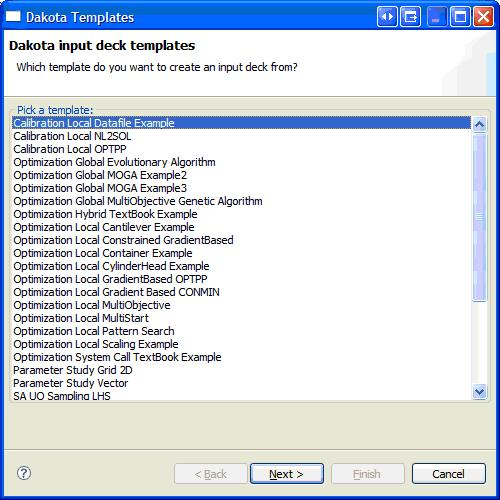
\includegraphics[scale=0.6]{images/jag_template1}
  \caption{A list of DAKOTA input file templates in JAGUAR}
  \label{fig:input:jag_template1}
\end{figure}
\begin{figure}
  \centering
  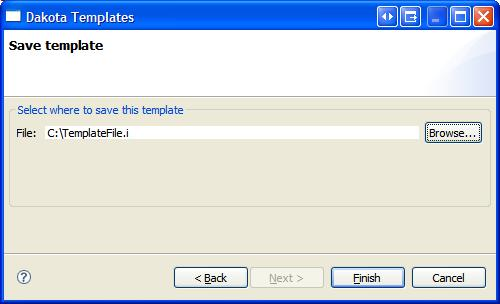
\includegraphics[scale=0.6]{images/jag_template2}
  \caption{Specifying a location for saving an input file generated
    from a template.}
  \label{fig:input:jag_template2}
\end{figure}

\newpage
\subsection{Brief tutorial on how to use JAGUAR}

Here we provide a simple example originating from the input file dakota\_rosebrock\_2d.in that can be found in the examples/tutorial
directory of the Dakota distributions. To familiarize with JAGUAR's basics please follow the steps described below.

Start Jaguar

In the Welcome screen, select ``Configure Jaguar'' or click {\bf Window $\rightarrow$ Preferences $\rightarrow$ Jaguar} (see Figure~\ref{fig:input:0Preferences}).
\begin{itemize}
\item Under Jaguar options, provide your paths for ``DAKOTA executable'' (this is the full path for the Dakota executable file you will use to run Dakota), ``Save path'' (this is the full path for the directory you wish to save your input files in) and ``Templates path'' (this is the full path for the directory you wish to save your own Dakota Templates in).
\item Select ``OK''.
\end{itemize}
\begin{figure}[htbp]
  \centering
  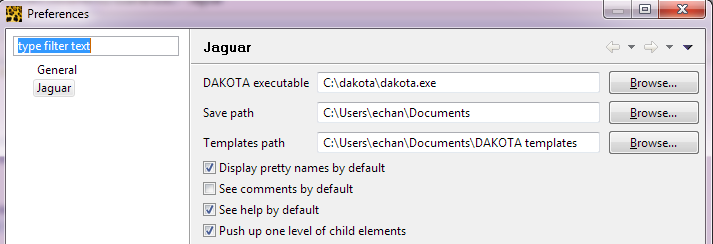
\includegraphics[scale=0.6]{images/0Preferences}
  \caption{JAGUAR Preferences}
  \label{fig:input:0Preferences}
\end{figure}

{\bf File $\rightarrow$ New $\rightarrow$ DAKOTA input file from template}
\begin{itemize}
\item Do either of the following:
\begin{enumerate}
\item Type ``tutorial'' in the quick search bar and select ``Tutorial Rosenbrock''
\item Navigate down and select ``Tutorial Rosenbrock''
\end{enumerate}
\item A preview of the template file should be visible, see Figure~\ref{fig:input:1tutorial}.
\item Select ``Next''
\item Specify a filename such as ``rosenbrock.i''
\item Select ``Finish''
\end{itemize}
\begin{figure}[htbp]
  \centering
  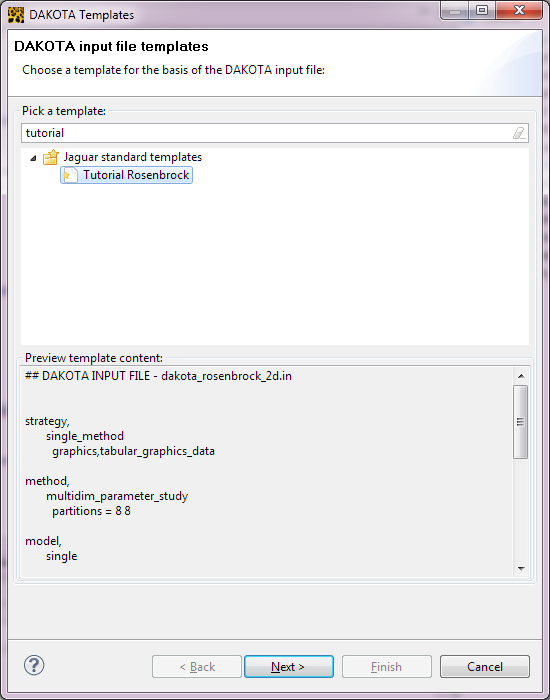
\includegraphics[scale=0.6]{images/1tutorial}
  \caption{DAKOTA input file templates}
  \label{fig:input:1tutorial}
\end{figure}


As in Figure~\ref{fig:input:2rosenbrockfile} notice the following:
\begin{itemize}      
\item There are errors with \texttt{direct} and \texttt{analysis\_driver}. (Note: These error messages occur because there is a limitation in the ordering of keywords currently parsed for JAGUAR from DAKOTA. We plan to address this issue in future JAGUAR releases. For DAKOTA these are valid keywords). 
\item Mouse over and see the tooltip errors.
\item Mouse over other keywords to see additional information.
\item To run the advanced parsing engine and to format the text, press Ctrl-Shift-F or {\bf Edit $\rightarrow$ Format}. Observe the updated rosenbrock\_2d template input file in Figure~\ref{fig:input:3fixed}. 
\item You can always Undo (Ctrl-Z or {\bf Edit $\rightarrow$ ''Undo Typing''}) and Redo (Ctrl-Y or {\bf Edit $\rightarrow$ ''Redo Typing''}) to compare.
\end{itemize}
\begin{figure}[htbp]
  \centering
  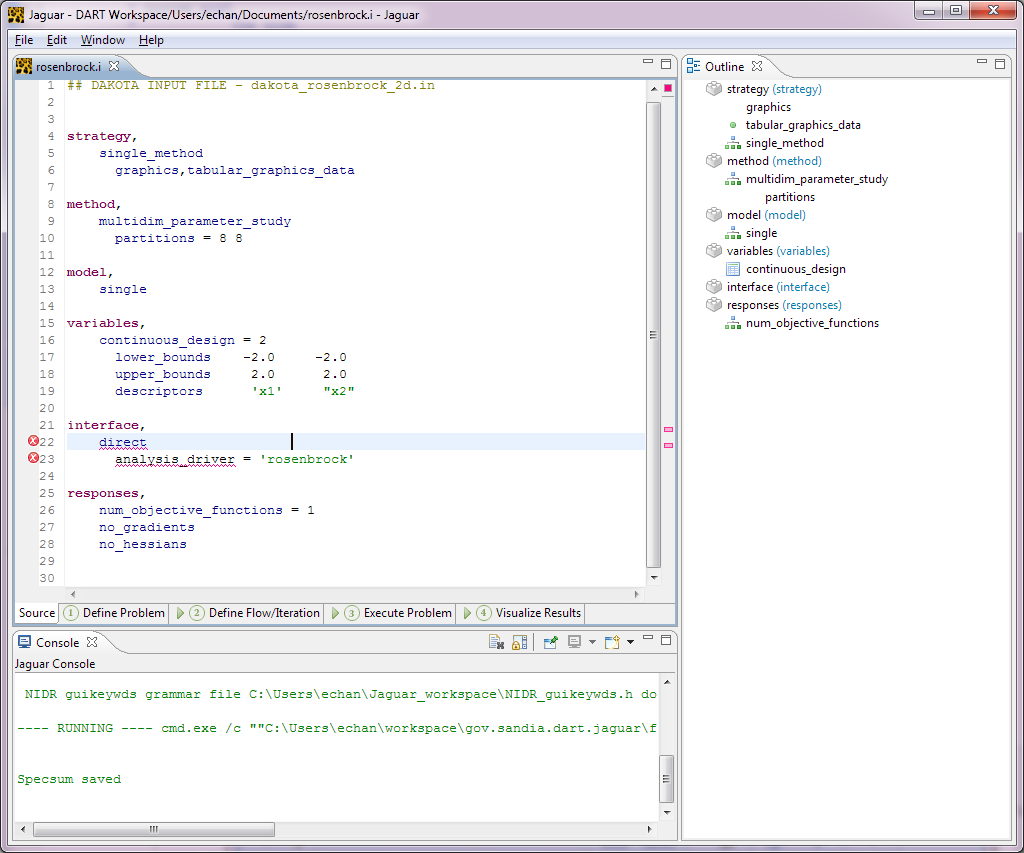
\includegraphics[scale=0.6]{images/2rosenbrockfile}
  \caption{rosenbrock\_2d input file}
  \label{fig:input:2rosenbrockfile}
\end{figure}

In Figure~\ref{fig:input:3fixed} notice the following:
\begin{itemize}
\item cleaner look (unnecessary spaces and newlines removed)
\item \texttt{analysis\_driver} replaced with \texttt{analysis\_drivers} (JAGUAR specific keyword correction)
\item \texttt{direct} now a sub-element of \texttt{analysis\_drivers} (JAGUAR specific keyword correction)
\item double quoted ``x2'' replaced with single quoted 'x2' (uniform)
\end{itemize}
\begin{figure}[htbp]
  \centering
  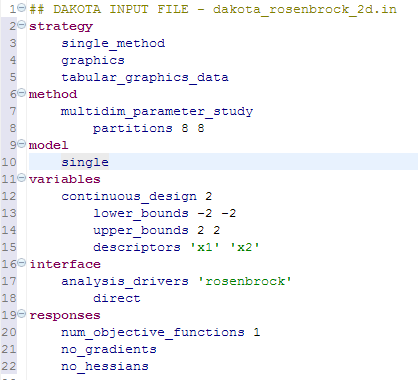
\includegraphics[scale=0.6]{images/3fixed}
  \caption{``Updated'' rosenbrock\_2d template input file after using the advanced parsing engine}
  \label{fig:input:3fixed}
\end{figure}      


To execute click the tab ``(3) Execute Problem'' at the bottom (see previously in Figure~\ref{fig:input:jag_execute}). 
In Figure~\ref{fig:input:5Visualize} notice the following:
\begin{itemize}
\item Actual DAKOTA command (in green) just ran.
\item Output of DAKOTA's check run below.
\end{itemize}
\begin{figure}[htbp]
  \centering
  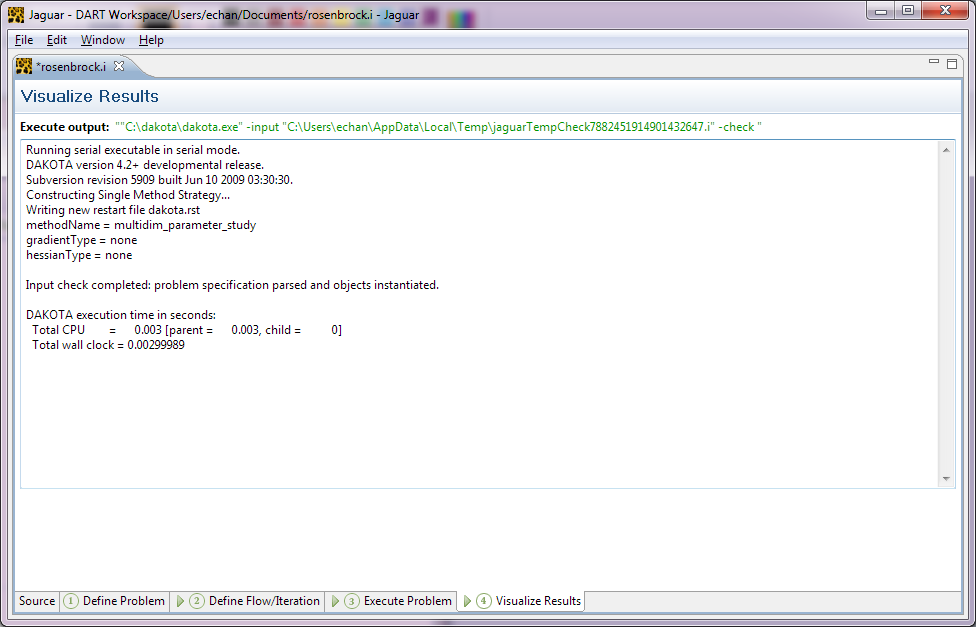
\includegraphics[scale=0.6]{images/5Visualize}
  \caption{``Visualize Results'' tab}
  \label{fig:input:5Visualize}
\end{figure}


Now go back to the Source (1st tab):
\begin{itemize}
\item Find tabular\_graphics\_data (around line 5), create a new line below and press Ctrl-Space. Notice a list of keywords are listed in a dropdown, see Figure~\ref{fig:input:6Autocomplete}.
\item Press up or down arrows to navigate.
\item Navigate to ``output\_precision'' but DO NOT press Enter.
\begin{figure}[htbp]
  \centering
  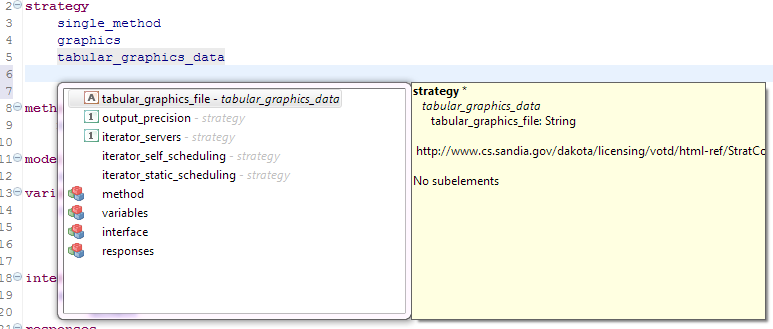
\includegraphics[scale=0.6]{images/6Autocomplete}
  \caption{}
  \label{fig:input:6Autocomplete}
\end{figure}
\begin{itemize}
\item Notice that strategy is highlighted in the text, and also listed next to output\_precision. Auto-completing keywords are sorted backwards, meaning they keywords at the top are the closest matching keywords. This helps you discover relevant keywords.
\end{itemize}
\item Select output\_precision
\item Notice auto-complete types in an equal ``='' for you to remind you to enter a value.
\item Type in ``notinteger''.
\item Notice red underline shows an error has occurred.
\item Mouse over it (as in Figure~\ref{fig:input:7texterror}).
\begin{figure}[htbp]
  \centering
  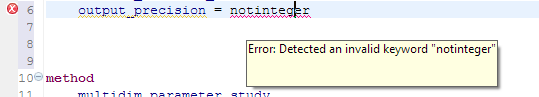
\includegraphics[scale=0.6]{images/7texterror}
  \caption{Text error detailed message}
  \label{fig:input:7texterror}
\end{figure}
\item Correct by replacing it with a valid integer
\item On the next line, type in ``iterato''.
\item Right after the ``o'' in ``iterato'', press Ctrl-Space.
\item Notice auto-completion can also finish off half completed keywords. Pick one (see Figure~\ref{fig:input:8iterato}).
\end{itemize}
\begin{figure}[htbp]
  \centering
  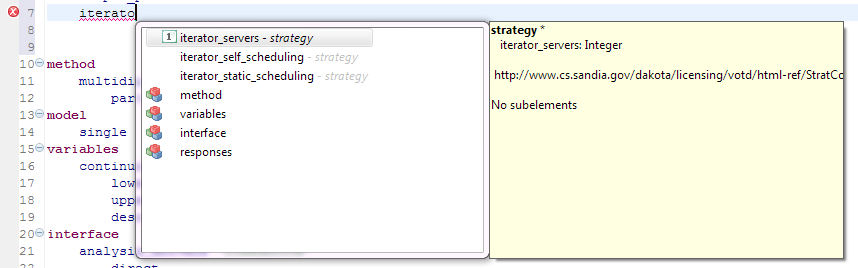
\includegraphics[scale=0.6]{images/8iterato}
  \caption{Auto-completion window}
  \label{fig:input:8iterato}
\end{figure}


Save this corrected rosenbrock file as your own template (Figure~\ref{fig:input:9SaveAsTemplate}):
{\bf File $\rightarrow$ Save As Template}
\begin{itemize}
\item Notice: this path is specified in the Jaguar Preferences you had set earlier.
\item Name it ``Rosenbrock Fixed''
\item Click ``Save''
\end{itemize} 
\begin{figure}[htbp]
  \centering
  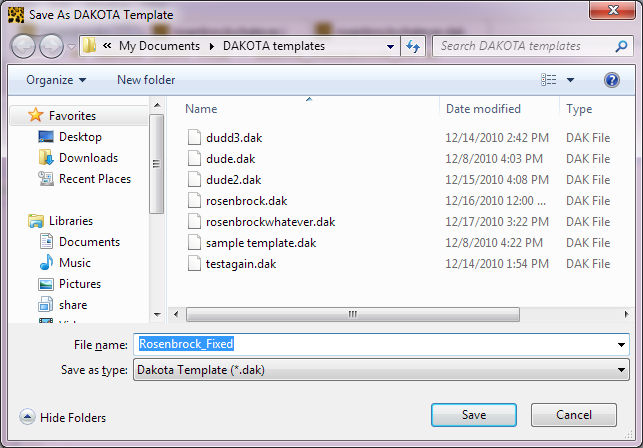
\includegraphics[scale=0.6]{images/9SaveAsTemplate}
  \caption{Save As DAKOTA Template Window}
  \label{fig:input:9SaveAsTemplate}
\end{figure}


Close all files (Ctrl-Shift-W) or {\bf File $\rightarrow$ ''Close All''}. No need to save changes.


Click on {\bf File $\rightarrow$ New $\rightarrow$ DAKOTA input file from template} 
\begin{itemize}
\item Do either of the following:
\begin{enumerate}
\item Type ``Fixed'' in the quick search bar and select ``Rosenbrock Fixed''
\item Navigate down and select ``Rosenbrock Fixed''
\end{enumerate}
\begin{figure}[htbp]
  \centering
  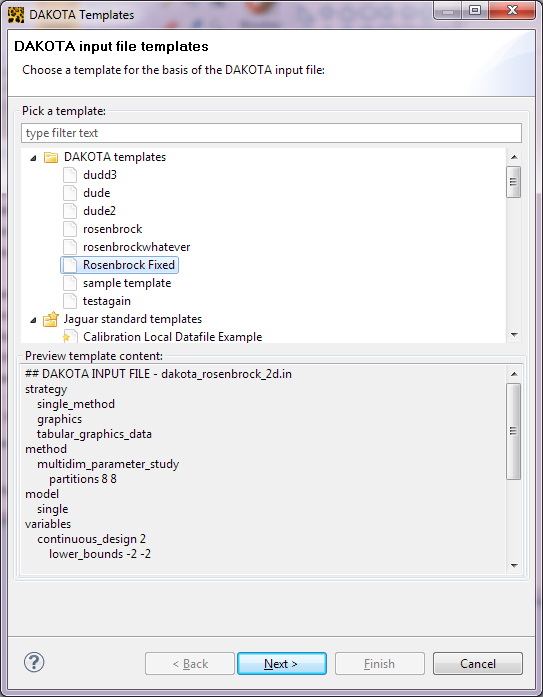
\includegraphics[scale=0.6]{images/10Template_Rosenbrock}
  \caption{Rosenbrock Fixed DAKOTA Template}
  \label{fig:input:10Template_Rosenbrock}
\end{figure}

\item Notice (see Figure~\ref{fig:input:10Template_Rosenbrock}) that:
\begin{enumerate}
\item This time we are creating an input file from a user-created template.
\item User-created templates do not have stars on them and are listed at the top.
\end{enumerate} 
\item A preview of the template file should be visible.
\item Select ``Next''
\item Specify a filename such as ``rosenbrock\_fixed.i'' 
\item Select ``Finish''
\end{itemize}


This completes the basic tutorial of JAGUAR 2.1.

\subsection{Troubleshooting}

In case of errors, please try these options:
\begin{enumerate}
\item  Check if your Java version is supported: In a Command Prompt type``java -version''. You should have at least Java 1.5
\item  If there exists a corrupted JAGUAR workspace, remove the workspace (User\_folder \textgreater Jaguar\_workspace).
\item  Enable Error Log: {\bf Window $\rightarrow$ Show View $\rightarrow$ Error Log} (see Figure~\ref{fig:input:11ShowView}).
\end{enumerate}

\begin{figure}[htbp]
  \centering
  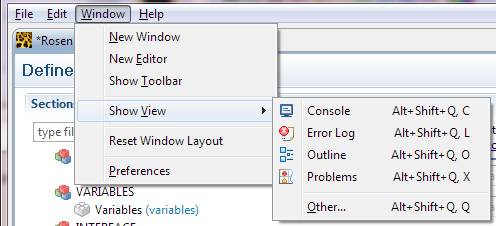
\includegraphics[scale=0.6]{images/11ShowView}
  \caption{Enabling Jaguar Error Log}
  \label{fig:input:11ShowView}
\end{figure}


Send any errors listed to our support email (jaguar-help@sandia.gov).

\newpage
\section{Data Imports}\label{input:import}

The DAKOTA input file and/or command line may identify additional
files used to import data into DAKOTA.

\subsection{AMPL algebraic mappings: stub.nl, stub.row, and stub.col}

As described in Section~\ref{interfaces:algebraic}, an AMPL
specification of algebraic input-to-output relationships may be
imported into DAKOTA and used to define or augment the mappings of a
particular interface.

\subsection{Genetic algorithm population import}

Genetic algorithms (GAs) from the JEGA and COLINY packages support a 
population import feature using the keywords 
\texttt{initialization\_type flat\_file = \emph{STRING}}.  This is 
useful for warm starting GAs from available data or previous runs.
Refer to the Method Specification chapter in the DAKOTA Reference
Manual~\cite{RefMan} for additional information on this specification.

\subsection{Least squares data import}

Least squares methods can read files of whitespace-separated
experimental data to difference with model results, with one
experimental data point given per model response returned to DAKOTA.
See~\ref{nls:examples} and the DAKOTA Reference Manual for further
details.

\subsection{PCE coefficient import}

Polynomial chaos expansion (PCE) methods compute coefficients for
response expansions which employ a basis of multivariate orthogonal
polynomials.  Normally, the \texttt{polynomial\_chaos} method
calculates these coefficients based either on a spectral projection or
a linear regression (see Section~\ref{uq:expansion}).  However,
DAKOTA also supports the option of importing a set of response PCE
coefficients based on the specification
\texttt{expansion\_import\_file = \emph{STRING}}.  This is useful for
evaluating moments analytically or computing probabilities numerically
from a known response expansion.  Refer to the Method Specification
chapter in the DAKOTA Reference Manual~\cite{RefMan} for additional
information on this specification.

\subsection{Surrogate construction from data files}

Global data fit surrogates may be constructed from a variety of
data sources.  One of these sources is an auxiliary data file,
as specified by the keywords 
\texttt{reuse\_samples samples\_file = \emph{STRING}}.  Refer to the 
Model Specification chapter in the DAKOTA Reference 
Manual~\cite{RefMan} for additional information on this specification.

\subsection{Variables/responses import to post-run}

The post-run mode (supported only for sampling, parameter study, and
DACE methods) requires specification of a file containing parameter
and response data in columnar format.  Columns for variables are
followed by those for responses, with an ignored header row of labels
and then one row per evaluation.  Typically this file would be
generated by executing \texttt{dakota -i dakota.in -pre\_run
::variables.dat} and then adding columns of response data to
variables.dat to make varsresponses.dat.  The file is specified as
follows at the command line:
\begin{small}
\begin{verbatim}
    dakota -i dakota.in -post_run varsresponses.dat::
\end{verbatim}
\end{small}

%PCE coefficients
